\section{Tooling}\label{sec:tooling}

\subsection{ATM}\label{sec:atm}
ATM is a model-based testing web application, developed in the Ruby on Rails framework. It has been used to test the software of several big companies in the Netherlands since 2006. It is under continuous development by Axini.

The UML sequence diagram for ATM is shown in Figure~\ref{fig:axini_tool}.

\begin{figure}[h]
  \begin{center}
    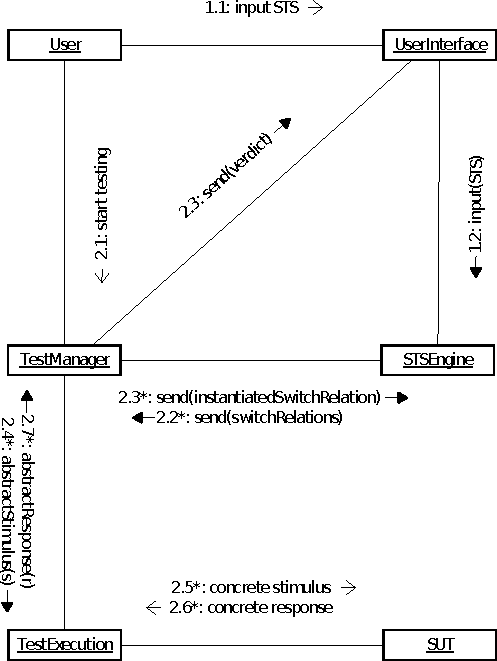
\includegraphics[width=\textwidth]{atm-diagram.pdf}
  \end{center}
  \caption{ATM sequence diagram}
  \label{fig:axini_tool}
\end{figure}

The tool functions as follows: 
\begin{enumerate}
  \item An STS is given to an STS Engine, which keeps track of the current location and variables. The user starts the test and gives a `depth', indicating how many stimuli should be tested. The variable $i$ stands for the current iteration of $loop$ and is initially set to $0$. The variable $verdict$ is initially set to $'pass'$.
  \item The STS Engine gives the possible switch relations from the current location to the Test Manager. It chooses an enabled switch relation based on a test strategy, which can be a random strategy or a strategy designed to obtain a high location/switch relation coverage. The valuation of the variables in the guard are also chosen by a test strategy, which can be a random strategy or a strategy using boundary-value analysis. The choice is represented by an instantiated switch relation.
  \item The instantiated switch relation is given to the Test Execution component as an \textit{abstract stimulus}. The term abstract indicates that the instantiated switch relation is an abstract representation of some computation steps taken in the SUT. For instance, a transition with label `?connect' is an abstract stimulus of the actual setup of a TCP connection between two distributed components of the SUT. 
  \item The translation of an abstract stimulus to a concrete stimulus is done by the Adapter. This component has to be programmed by the tester such that the abstract stimulus is correctly translated to a concrete stimulus. This component provides the stimulus to the SUT. When the SUT responds, the Adapter translates this response to an abstract response. For instance, the Adapter receives an HTTP response that the TCP connect was succesful. This is a concrete response, which the Adapter translates to an abstract response, such as an instantiated switch relation with gate `!ok'. The SUT can also give multiple responses. As with the stimuli, the tester has to program the translation from concrete responses to abstract responses. The Test Manager is notified with these abstract responses.
  \item The Test Manager updates the STS engine with the chosen abstract stimuli and received abstract responses. If this is possible according to the STS, a pass verdict is given, otherwise a fail verdict is given. The Test Manager updates the $verdict$ variable accordingly. The loop continues as long as all responses are according to the specification and the required number of tested stimuli has not been reached. The test is stopped at a fail verdict, because the SUT has entered an invalid state and the STS engine cannot give possible switch relations any more. For instance, an error could have occurred, which is an invalid response and makes continuing impossible.
  \item When the Test Manager finishes it gives a pass verdict for this test if all verdicts given by the STS engine were a pass verdict. Otherwise, the result is a fail verdict. Also a trace is given of all chosen and observed instantiated switch relations. This can be used to calculate coverage information for the test and to allow the SUT or the STS to be fixed in case of a fail verdict.
\end{enumerate}

\subsection{GROOVE}\label{sec:descriptiongroove}
GROOVE is an open source, graph-based modelling tool in development at the University of Twente since 2004~\cite{Rensink:GROOVE}. It has been applied to several case studies, such as model transformations and security and leader election protocols~\cite{Ghamarian:GROOVE}. The UML sequence diagram for GROOVE is shown in Figure~\ref{fig:groove_tool}.

\begin{figure}[h]
  \begin{center}
    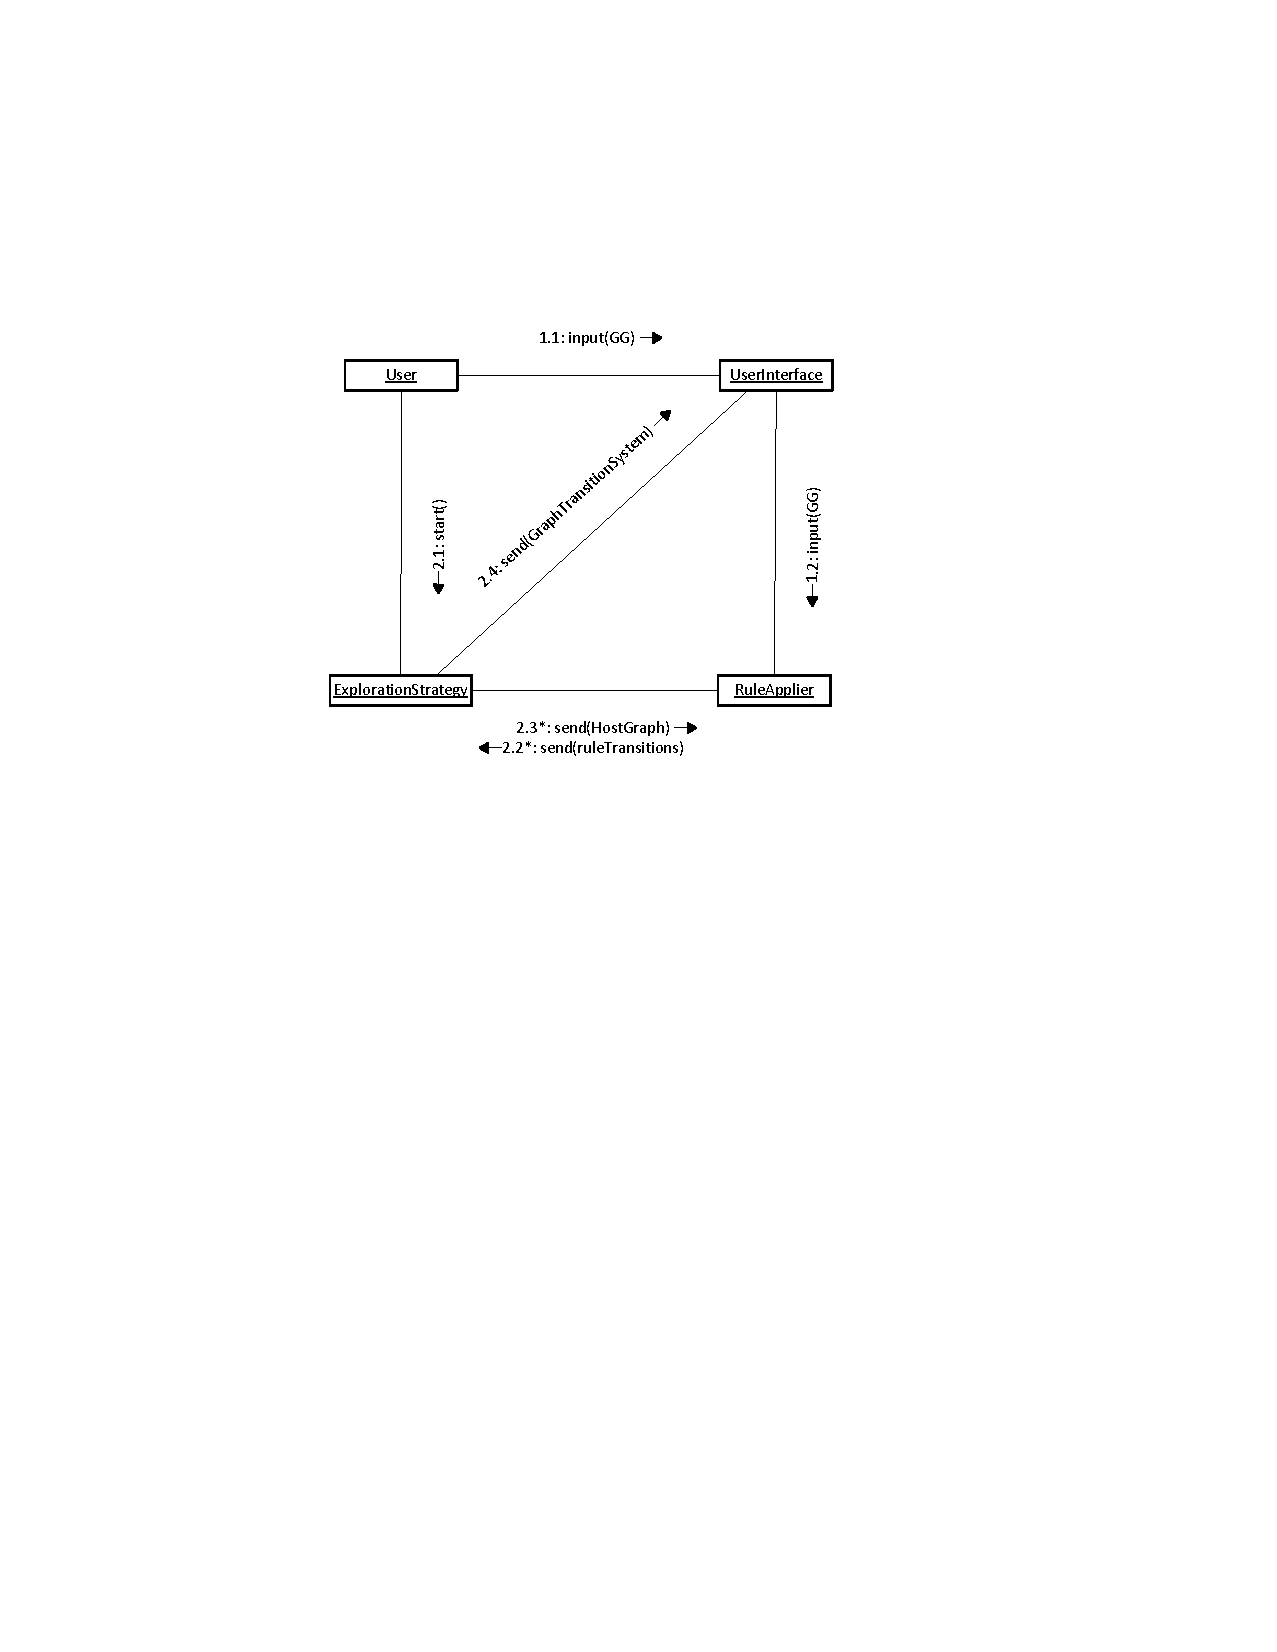
\includegraphics[width=0.75\textwidth]{groove-diagram.pdf}
  \end{center}
  \caption{GROOVE sequence diagram}
  \label{fig:groove_tool}
\end{figure}

The tool functions as follows:
\begin{enumerate}
\item A graph grammar is given as input to a RuleApplier component, which determines the possible rule transitions.
\item The user starts an ExplorationStrategy. This strategy explores all possible host graphs and rule transitions. The possible rule transitions from the initial graph state are obtained from the RuleApplier and a rule transition is chosen, based on the exploration strategy. The target host graph of the chosen rule transition is again given to the RuleApplier until no more new host graphs can be explored.
\item The ExplorationStrategy returns the explored GTS to the UserInterface.
\end{enumerate}

\subsection{GROOVE visual elements}
\paragraph*{Labels and flags}
Nodes in GROOVE have several kinds of labels: regular labels, type labels and flags. Figure \ref{fig:flags} shows a node with a type label (bold), two flags (italic) and two regular labels. Nodes in GROOVE can have one type, indicated by the type label. Typing is not explained further in this report\footnote{See the documentation of GROOVE for more information: http://groove.cs.utwente.nl/doc/}. A node can have multiple regular labels and flags. 

\begin{figure}[h]
  \begin{center}
    % To use this figure in your LaTeX document
% import the package groove/resources/groove2tikz.sty
%
% Special colors
\begin{tikzpicture}[
% Special color styles
scale=\tikzscale]
\node[node] (n0)  at (0.820, -0.910) {\ml{\textbf{Type}\\\textit{flag1}\\\textit{flag2}\\label1\\label2}};
\userdefinedmacro
\end{tikzpicture}
\renewcommand{\userdefinedmacro}{\relax}

  \end{center}
  \caption{GROOVE labels and flags}
  \label{fig:flags}
\end{figure}

\paragraph*{Rule node matching}
Nodes in a rule graph in GROOVE can also match each other, by connecting them with an equals `=' labelled edge. This means that any images of both nodes have to be the same. Figure \ref{fig:node_match1} shows an example of this. Nodes in a rule graph in GROOVE can also explicitly not match each other, by connecting them with an not-equals `!=' labelled edge. This means that any images of both nodes cannot be the same. Figure \ref{fig:node_match2} shows an example of this.

\begin{figure}[h]
  \begin{center}
    \subfloat[Matching rule nodes]{\label{fig:node_match1}% To use this figure in your LaTeX document
% import the package groove/resources/groove2tikz.sty
%
% Special colors
\begin{tikzpicture}[
% Special color styles
scale=\tikzscale]
\node[node] (n0)  at (0.900, -0.850) {\ml{node1}};
\node[node] (n1)  at (1.790, -0.850) {\ml{node2}};
\path[edge, -](n0.east |- 1.790, -0.850) -- node[lab]{\textit{=}} (n1) ;
\userdefinedmacro
\end{tikzpicture}
\renewcommand{\userdefinedmacro}{\relax}
}\hspace{20px}
    \subfloat[Non-matching rule nodes]{\label{fig:node_match2}% To use this figure in your LaTeX document
% import the package groove/resources/groove2tikz.sty
%
% Special colors
\begin{tikzpicture}[
% Special color styles
scale=\tikzscale]
\node[node] (n1)  at (1.790, -0.850) {\ml{node2}};
\node[node] (n0)  at (0.900, -0.850) {\ml{node1}};
\path[edge, -](n0.east |- 1.790, -0.850) -- node[lab]{\textit{!=}} (n1) ;
\userdefinedmacro
\end{tikzpicture}
\renewcommand{\userdefinedmacro}{\relax}
}
  \end{center}
  \caption{Node matching in GROOVE rule graphs}
  \label{fig:node_match}
\end{figure}

\paragraph*{Colors}
Rule graphs in GROOVE combine $\mathit{LHS}$, $\mathit{RHS}$ and $\mathit{NAC}$ into one rule graph. The colors on the nodes and edges in GROOVE rules represent whether they belong to the $\mathit{LHS}$, $\mathit{RHS}$ or $\mathit{NAC}$ of the rule. See Figure \ref{fig:colors} for an example.
\begin{enumerate}
  \item normal line (black): This node or edge is part of both the $\mathit{LHS}$ and $\mathit{RHS}$.
  \item dotted line (red): This node or edge is part of the $\mathit{NAC}$ only.\marginpar{dotted line is niet helemaal correct beter woord?}
  \item thick line (green): This node or edge is part of the $\mathit{RHS}$ only.
  \item dashed line (blue): This node or edge is part of the $\mathit{LHS}$ only.
\end{enumerate}

\begin{figure}[h]
  \begin{center}
    % To use this figure in your LaTeX document
% import the package groove/resources/groove2tikz.sty
%
% Special colors
\begin{tikzpicture}[
% Special color styles
scale=\tikzscale]
\node[node] (n0)  at (1.040, -0.990) {\ml{\textbf{LHS\_and\_RHS}}};
\node[nacnode] (n1)  at (2.380, -1.000) {\ml{NAC}};
\node[newnode] (n2)  at (1.050, -1.660) {\ml{\textbf{RHS}}};
\node[delnode] (n3)  at (2.380, -1.670) {\ml{\textbf{LHS}}};
\path[nacedge](n0.east |- 2.380, -1.000) -- node[naclab]{foo} (n1) ;
\path[deledge] (n0)  -- node[dellab]{bar} (n3) ;
\path[newedge](n0.south -| 1.050, -1.660) -- node[newlab]{baz} (n2) ;
\userdefinedmacro
\end{tikzpicture}
\renewcommand{\userdefinedmacro}{\relax}

  \end{center}
  \caption{GROOVE rule graph colors}
  \label{fig:colors}
\end{figure}

\paragraph*{Variable nodes and terms}
Variable nodes in GROOVE are represented by their type: `int', `bool', `real' and `string' for integer, boolean, real and string variables respectively. Figure \ref{fig:terms} shows two integer variable nodes and the constant integer node `1'. The diamond shaped node is a term node. It has two \textit{argument} edges $\pi_0, \pi_1$ and a \textit{result} edge `int:add'. The term represented here is the addition of two integers, the first one being an integer variable, the second being the number 1. When this rule matches a host graph, the target variable node of the result edge is set to the result of the term; in this case the image of the first variable node plus one.

\begin{figure}[h]
  \begin{center}
    % To use this figure in your LaTeX document
% import the package groove/resources/groove2tikz.sty
%
% Special colors
\begin{tikzpicture}[
% Special color styles
scale=\tikzscale]
\node[node] (n0)  at (0.860, -0.560) {\ml{\textbf{Node}}};
\node[node, attr] (n1)  at (0.850, -1.210) {\ml{\textbf{int}}};
\node[node, attr] (n2)  at (1.750, -0.550) {\ml{\textbf{int}}};
\node[node, prod] (n3)  at (1.750, -1.210){};
\node[node, attr] (n4)  at (2.400, -1.210) {\ml{1}};
\path[deledge](n0.south -| 0.850, -1.210) -- node[dellab]{x} (n1) ;
\path[newedge](n0.east |- 1.750, -0.550) -- node[newlab]{x} (n2) ;
\path[edge] (n3)  -- node[lab]{$\pi$0} (n1) ;
\path[edge] (n3)  -- node[lab]{$\pi$1} (n4) ;
\path[edge] (n3)  -- node[lab]{add} (n2) ;
\userdefinedmacro
\end{tikzpicture}
\renewcommand{\userdefinedmacro}{\relax}

  \end{center}
  \caption{Terms in GROOVE rule graphs}
  \label{fig:terms}
\end{figure}

\paragraph*{Term shorthand notation}
A rule node with an edge to a constant is shortened to a label on the node. Figure \ref{fig:shorthand1} shows a node with an edge labelled `x' to the constant `1'. Figure \ref{fig:shorthand2} shows the shorthand notation of this edge as the label `x = 1' on the source node of the edge. Terms can also be shortened. The rule graph in Figure \ref{fig:terms} can be shortened to the rule graph in Figure \ref{fig:term_shorthand}.

\begin{figure}[h]
  \begin{center}
    \subfloat[edge to constant]{\label{fig:shorthand1}\parbox{80px}{\centering% To use this figure in your LaTeX document
% import the package groove/resources/groove2tikz.sty
%
% Special colors
\begin{tikzpicture}[
% Special color styles
scale=\tikzscale]
\node[node] (n0)  at (1.075, -0.735) {\ml{Node}};
\node[node, attr] (n1)  at (2.010, -0.725) {\ml{1}};
\path[edge](n0.east |- 2.010, -0.725) -- node[lab]{x} (n1) ;
\userdefinedmacro
\end{tikzpicture}
\renewcommand{\userdefinedmacro}{\relax}
}}\hspace{20px}
    \subfloat[shorthand notation]{\label{fig:shorthand2}\parbox{90px}{\centering% To use this figure in your LaTeX document
% import the package groove/resources/groove2tikz.sty
%
% Special colors
\begin{tikzpicture}[
% Special color styles
scale=\tikzscale]
\node[node] (n0)  at (1.080, -0.740) {\ml{\textbf{Node}\\x = 1}};
\userdefinedmacro
\end{tikzpicture}
\renewcommand{\userdefinedmacro}{\relax}
}}
  \end{center}
  \caption{Constant shorthand notation in GROOVE}
  \label{fig:shorthand}
\end{figure}

\begin{figure}[h]
  \begin{center}
    % To use this figure in your LaTeX document
% import the package groove/resources/groove2tikz.sty
%
% Special colors
\begin{tikzpicture}[
% Special color styles
scale=\tikzscale]
\node[node] (n0)  at (0.860, -0.560) {\ml{\textbf{Node}\\{\color{\green}x := x $+$ 1}}};
\userdefinedmacro
\end{tikzpicture}
\renewcommand{\userdefinedmacro}{\relax}

  \end{center}
  \caption{Term shorthand notation in GROOVE}
  \label{fig:term_shorthand}
\end{figure}

\paragraph*{Rule transition parameters}
Rule transitions can have parameters in GROOVE. Figure \ref{fig:transition_parameters_rule} shows a rule where the node variables have a number in the top right of the node. These numbers indicate that the value of the variables are placed as parameters on the rule transition, in the order indicated by the numbers. This rule matches the host graph in Figure \ref{fig:transition_parameters_host}. The result of applying the rule twice is the GTS in Figure \ref{fig:transition_parameters_gts}.

\begin{figure}[h]
  \begin{center}
    \subfloat[Rule graph]{\label{fig:transition_parameters_rule}% To use this figure in your LaTeX document
% import the package groove/resources/groove2tikz.sty
%
% Special colors
\begin{tikzpicture}[
% Special color styles
scale=\tikzscale]
\node[node, attr] (n4)  at (2.400, -1.210) {\ml{1}};
\node[node, prod] (n3)  at (1.750, -1.210){};
\node[node, attr] (n2)  at (1.750, -0.550) {\ml{\textbf{int}}};
\node[parnode] (n2p)  at (n2.north west) {1};
\node[node, attr] (n1)  at (0.850, -1.210) {\ml{\textbf{int}}};
\node[parnode] (n1p)  at (n1.north west) {0};
\node[node] (n0)  at (0.860, -0.560) {\ml{\textbf{Node}}};
\path[deledge](n0.south -| 0.850, -1.210) -- node[dellab]{x} (n1) ;
\path[newedge](n0.east |- 1.750, -0.550) -- node[newlab]{x} (n2) ;
\path[edge] (n3)  -- node[lab]{$\pi$0} (n1) ;
\path[edge] (n3)  -- node[lab]{$\pi$1} (n4) ;
\path[edge] (n3)  -- node[lab]{add} (n2) ;
\userdefinedmacro
\end{tikzpicture}
\renewcommand{\userdefinedmacro}{\relax}
}\hspace{20px}
    \subfloat[Host graph]{\label{fig:transition_parameters_host}% To use this figure in your LaTeX document
% import the package groove/resources/groove2tikz.sty
%
% Special colors
\begin{tikzpicture}[
% Special color styles
scale=\tikzscale]
\node[node] (n0)  at (0.860, -0.730) {\ml{\textbf{Node}\\x = 1}};
\userdefinedmacro
\end{tikzpicture}
\renewcommand{\userdefinedmacro}{\relax}
}\hspace{20px}
    \subfloat[GTS]{\label{fig:transition_parameters_gts}% To use this figure in your LaTeX document
% import the package groove/resources/groove2tikz.sty
%
% Special colors
\begin{tikzpicture}[
% Special color styles
scale=\tikzscale]
\node[node, start] (s0)  at (0.575, -0.165) {\ml{\textit{s0}}};
\node[node, open] (s1)  at (0.575, -0.895) {\ml{\textit{s1}}};
\node[node, open, bold] (s2)  at (0.575, -1.625) {\ml{\textit{s2}}};
\path[edge](s0.south -| 0.575, -0.895) -- node[lab]{add(1,2)} (s1) ;
\path[edge](s1.south -| 0.575, -1.625) -- node[lab]{add(2,3)} (s2) ;
\userdefinedmacro
\end{tikzpicture}
\renewcommand{\userdefinedmacro}{\relax}
}
  \end{center}
  \caption{Rule transition parameters in GROOVE}
  \label{fig:transition_parameters}
\end{figure}

\paragraph*{Quantification}
GROOVE supports quantification operations over nodes in rule graphs. Figure \ref{fig:quantification} shows a simple example. The `forall' operator here matches all nodes typed `Node'. GROOVE also supports the `exists' operator and nesting of operators, however this is out of scope for this report. The `forall' operator will be used in the model examples to perform operations over sets of nodes, such as in this rule: all self-edges labelled `x' on nodes typed `Node' are deleted from the host graph. 

\begin{figure}[h]
  \begin{center}
    % To use this figure in your LaTeX document
% import the package groove/resources/groove2tikz.sty
%
% Special colors
\begin{tikzpicture}[
% Special color styles
scale=\tikzscale]
\node[node] (n0)  at (0.970, -1.000) {\ml{\textbf{Node}}};
\node[quantnode] (n1)  at (0.950, -1.680) {\ml{$\forall$}};
\path[quantedge](n0.south -| 0.950, -1.680) -- node[lab]{@} (n1) ;
\path[deledge] (n0) .. controls (1.170, -0.700) and (1.120, -0.650) .. (1.120, -0.650).. controls (1.050, -0.580) and (0.930, -0.570) .. (0.870, -0.640).. controls (0.870, -0.640) and (0.800, -0.690) ..  (n0) ;
\node[dellab] at (0.990, -0.645){x};
\userdefinedmacro
\end{tikzpicture}
\renewcommand{\userdefinedmacro}{\relax}

  \end{center}
  \caption{An example of quantification in GROOVE}
  \label{fig:quantification}
\end{figure}

\subsection{Example GROOVE graph grammar}\label{sec:example_groove} 
The running example from Figure~\ref{fig:example_sts} is displayed as a graph grammar, as visualized in GROOVE, in Figure~\ref{fig:example_groove}. The $\mathit{LHS}$, $\mathit{RHS}$ and $\mathit{NAC}$ of a rule in GROOVE are visualized together in one graph. Figures~\ref{fig:example_groove_throw}, \ref{fig:example_groove_move} and \ref{fig:example_groove_next} show three rules. Figure~\ref{fig:example_groove_start} shows the start graph of the system.

\begin{figure}[h]
  \begin{center}
    \subfloat[The start graph]{\label{fig:example_groove_start}% To use this figure in your LaTeX document
% import the package groove/resources/groove2tikz.sty
%
% Special colors
\begin{tikzpicture}[
% Special color styles
scale=\tikzscale]
\node[node] (n0)  at (2.250, -0.605) {\ml{\textbf{Die}\\rolls = 0}};
\node[node] (n10)  at (3.560, -2.025) {\ml{\textbf{Location}}};
\node[node] (n9)  at (0.930, -1.985) {\ml{\textbf{Location}}};
\node[node] (n8)  at (2.200, -2.545) {\ml{\textbf{Location}}};
\node[node] (n11)  at (0.990, -0.600) {\ml{\textbf{Player}\\\textit{turn}\\id = 1}};
\node[node] (n7)  at (2.180, -1.465) {\ml{\textbf{Location}}};
\node[node] (n12)  at (3.550, -0.615) {\ml{\textbf{Player}\\id = 2}};
\path[edge](n11.south -| 0.930, -1.985) -- node[lab]{at} (n9) ;
\path[edge] (n10)  -- node[lab]{next} (n8) ;
\path[edge] (n9)  -- node[lab]{next} (n7) ;
\path[edge] (n8)  -- node[lab]{next} (n9) ;
\path[edge] (n7)  -- node[lab]{next} (n10) ;
\path[edge](n12.south -| 3.560, -2.025) -- node[lab]{at} (n10) ;
\userdefinedmacro
\end{tikzpicture}
\renewcommand{\userdefinedmacro}{\relax}
}\quad \\
    \subfloat[The throw rule]{\label{fig:example_groove_throw}% To use this figure in your LaTeX document
% import the package groove/resources/groove2tikz.sty
%
% Special colors
\begin{tikzpicture}[
% Special color styles
scale=\tikzscale]
\node[node] (n1)  at (0.545, -0.470) {\ml{\textbf{Player}\\\textit{turn}}};
\node[node] (n5)  at (1.595, -1.295) {\ml{\textbf{Die}}};
\node[nacnode, attr] (n2)  at (0.495, -1.325) {\ml{\textbf{int}}};
\node[node, attr] (n4)  at (1.605, -0.405) {\ml{\textbf{int}}};
\node[parnode] (n4p)  at (n4.north west) {0};
\path[newedge](n1.east |- 1.605, -0.405) -- node[newlab]{throws} (n4) ;
\path[edge](n5.north -| 1.605, -0.405) -- node[lab]{canThrow} (n4) ;
\path[nacedge](n1.south -| 0.495, -1.325) -- node[naclab]{throws} (n2) ;
\userdefinedmacro
\end{tikzpicture}
\renewcommand{\userdefinedmacro}{\relax}
}\hspace{10px}
    \subfloat[The move rule]{\label{fig:example_groove_move}% To use this figure in your LaTeX document
% import the package groove/resources/groove2tikz.sty
%
% Special colors
\begin{tikzpicture}[
% Special color styles
scale=\tikzscale]
\node[node] (n3)  at (2.840, -0.970) {\ml{\textbf{Die}\\{\color{\green}rolls := rolls $-$ 1}\\rolls $\>$ 0}};
\node[node] (n1)  at (1.540, -1.925) {\ml{\textbf{Location}}};
\node[node] (n0)  at (1.460, -0.970) {\ml{\textbf{Player}\\\textit{turn}}};
\node[node] (n2)  at (2.760, -1.915) {\ml{\textbf{Location}}};
\node[node, attr] (n4)  at (1.480, -0.400) {\ml{\textbf{int}}};
\node[parnode] (n4p)  at (n4.north west) {0};
\path[newedge] (n0)  -- node[newlab]{at} (n2) ;
\path[deledge](n0.south -| 1.540, -1.925) -- node[dellab]{at} (n1) ;
\path[edge](n1.east |- 2.760, -1.915) -- node[lab]{next} (n2) ;
\path[edge](n0.east |- 2.840, -0.970) -- node[lab]{throws} (n3) ;
\path[edge](n0.north -| 1.480, -0.400) -- node[lab]{id} (n4) ;
\userdefinedmacro
\end{tikzpicture}
\renewcommand{\userdefinedmacro}{\relax}
}\hspace{10px}
    \subfloat[The next turn rule]{\label{fig:example_groove_next}% To use this figure in your LaTeX document
% import the package groove/resources/groove2tikz.sty
%
% Special colors
\begin{tikzpicture}[
% Special color styles
scale=\tikzscale]
\node[node] (n0)  at (1.090, -0.650) {\ml{\textbf{Player}\\{\color{\blue}\textit{$-$ turn}}}};
\node[node] (n2)  at (2.050, -0.660) {\ml{\textbf{Player}\\{\color{\green}\textit{$+$ turn}}}};
\node[node] (n3)  at (1.080, -1.730) {\ml{\textbf{Die}\\rolls = 0}};
\path[edge, -](n0.east |- 2.050, -0.660) -- node[lab]{\textit{!=}} (n2) ;
\path[deledge](n0.south -| 1.080, -1.730) -- node[dellab]{throws} (n3) ;
\userdefinedmacro
\end{tikzpicture}
\renewcommand{\userdefinedmacro}{\relax}
}
  \end{center}
  \caption{The graph grammar of the board game example in Figure~\ref{fig:example_sts}}
  \label{fig:example_groove}
\end{figure}

The rules can be described as follows:
\begin{enumerate}
  \item~\ref{fig:example_groove_throw}: `if a player has the turn and he has not thrown the die yet, he may do so.'
  \item~\ref{fig:example_groove_move}: `if a player has the turn and he has thrown the die and this number is larger than zero, he may move one place and then it is as if he has thrown one less.'
  \item~\ref{fig:example_groove_next}: `if a player has finished moving (number thrown is zero), the next player receives the turn.'
\end{enumerate}

The graph is transformed after the rule is applied. The resulting graph after the transformation is the new state of the system and the rule is the transition from the old state (the graph as it was before the rule was applied) to the new state. Figure~\ref{fig:gts_example} shows the IOGTS of one \textit{?throws} rule application on the start graph. Note that the \textit{?throws} is an input, as indicated by the `?'. State $s_1$ is a representation of the graph in Figure~\ref{fig:example_groove_start}. Figure~\ref{fig:target_graph_state} shows the graph represented by $s_2$.

\begin{figure}[h]
  \begin{center}
    % To use this figure in your LaTeX document
% import the package groove/resources/groove2tikz.sty
%
% Special colors
\begin{tikzpicture}[
% Special color styles
scale=\tikzscale]
\node[node, start] (s0)  at (0.560, -0.155) {\ml{\textit{s0}}};
\node[node, open, bold] (s1)  at (0.565, -0.865) {\ml{\textit{s1}}};
\path[edge](s0.south -| 0.565, -0.865) -- node[lab]{throws?(2)} (s1) ;
\userdefinedmacro
\end{tikzpicture}
\renewcommand{\userdefinedmacro}{\relax}

  \end{center}
  \caption{The GTS after one rule application on the board game example in Figure~\ref{fig:example_groove}}
  \label{fig:gts_example}
\end{figure}

\begin{figure}[h]
  \begin{center}
    % To use this figure in your LaTeX document
% import the package groove/resources/groove2tikz.sty
%
% Special colors
\begin{tikzpicture}[
% Special color styles
scale=\tikzscale]
\node[node] (n12)  at (5.615, -0.525) {\ml{\textbf{Player}}};
\node[node] (n7)  at (4.245, -1.375) {\ml{\textbf{Location}}};
\node[node] (n11)  at (3.055, -0.520) {\ml{\textbf{Player}\\\textit{turn}\\throws = 2}};
\node[node] (n8)  at (4.265, -2.455) {\ml{\textbf{Location}}};
\node[node] (n9)  at (2.995, -1.895) {\ml{\textbf{Location}}};
\node[node] (n10)  at (5.625, -1.935) {\ml{\textbf{Location}}};
\node[node] (n0)  at (1.585, -0.865) {\ml{\textbf{Die}\\canThrow = 1\\canThrow = 2\\canThrow = 3\\canThrow = 4\\canThrow = 5\\canThrow = 6}};
\path[edge] (n8)  -- node[lab]{next} (n9) ;
\path[edge](n12.south -| 5.625, -1.935) -- node[lab]{at} (n10) ;
\path[edge] (n7)  -- node[lab]{next} (n10) ;
\path[edge](n11.south -| 2.995, -1.895) -- node[lab]{at} (n9) ;
\path[edge] (n9)  -- node[lab]{next} (n7) ;
\path[edge] (n10)  -- node[lab]{next} (n8) ;
\userdefinedmacro
\end{tikzpicture}
\renewcommand{\userdefinedmacro}{\relax}

  \end{center}
  \caption{The graph of state $s2$ in Figure~\ref{fig:gts_example}}
  \label{fig:target_graph_state}
\end{figure}